% Drawing 144/03-7 -- folder 144, batch 03, archive page 56 (PDF page 57).
% Transcription: Un sommet marqué $0$ au bord de $K$, d'où partent des arêtes vers des sommets $0$ et $\infty$ ; trois boucles fines emboîtées autour de l'arête qui aboutit en ce sommet, étiquetées $\tau_{0}r$, $r$ et $\tau_{\infty}\tau_{0}r = \tau_{1}\tau_{0}r$ (lecture douteuse), avec flèches de rotation.
% Kind: vertex of K with nested loops of frames. Method 2 (schematic redraw from the facsimile). Status: ok.
% Notes: A vertex 0 at the boundary of K with its edges (midpoints 1) to vertices 0, and the edge to the vertex infinity; three nested thin loops round that edge carry tau_0 r, r and tau_infty tau_0 r = tau_1 tau_0 r (reading doubtful, as in the transcription). Rotation arrows abbreviated.
% Coordinates: 1 unit = 1 mm = 1/100 of the crop width (bbox in page fractions: [0.28, 0.53, 0.6, 0.68]).
% Redrawn by Claude (claude-opus-5-5), issue #73, 2026-11-07; not checked by a human; not compiled (no TeX in the session).
% Rights: reproduces part of the work -- behind RENDER_TRANSCRIPTS, never published by itself.
\documentclass[tikz,border=3pt]{standalone}
\usepackage{amsmath,amssymb}
\usetikzlibrary{patterns,arrows.meta}
\tikzset{pencil/.style={black!45}, struck/.style={black!35}, mark/.style={circle,draw,inner sep=1.3pt}, pt/.style={circle,fill,inner sep=0.9pt}, opt/.style={circle,draw,fill=white,inner sep=1.1pt}}
\begin{document}
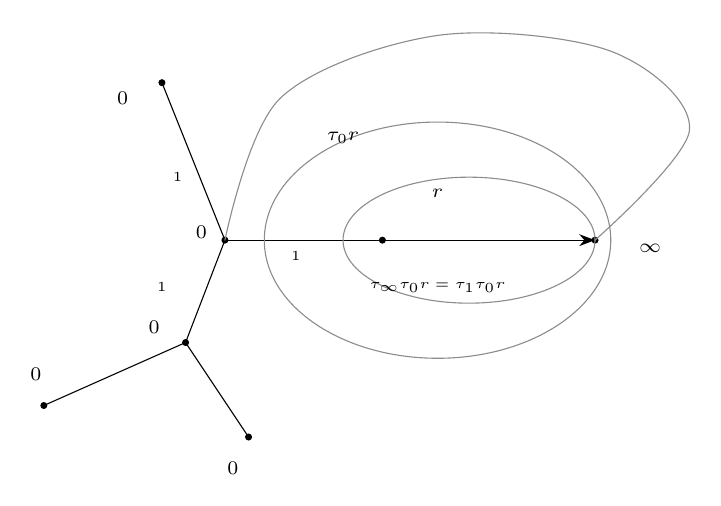
\begin{tikzpicture}[x=1mm,y=1mm,line cap=round,line join=round,font=\scriptsize]
\draw (25,-10) -- (33,-30);
\draw (33,-30) -- (28,-43);
\draw (10,-51) -- (28,-43) -- (36,-55);
\draw[-{Stealth[length=2mm]}] (33,-30) -- (80,-30);
\node[pt] at (25,-10) {};
\node[pt] at (33,-30) {};
\node[pt] at (28,-43) {};
\node[pt] at (10,-51) {};
\node[pt] at (36,-55) {};
\node[pt] at (80,-30) {};
\node[pt] at (53,-30) {};
\node[inner sep=1pt] at (20,-12) {\scriptsize $0$};
\node[inner sep=1pt] at (30,-29) {\scriptsize $0$};
\node[inner sep=1pt] at (24,-41) {\scriptsize $0$};
\node[inner sep=1pt] at (9,-47) {\scriptsize $0$};
\node[inner sep=1pt] at (34,-59) {\scriptsize $0$};
\node[inner sep=1pt] at (27,-22) {\tiny $1$};
\node[inner sep=1pt] at (25,-36) {\tiny $1$};
\node[inner sep=1pt] at (42,-32) {\tiny $1$};
\node[inner sep=1pt] at (87,-31) {\scriptsize $\infty$};
\draw[pencil] plot[smooth, tension=0.55] coordinates {(33,-30) (40,-12) (60,-4) (82,-6) (92,-16) (80,-30)};
\draw[pencil] (60,-30) ellipse[x radius=22, y radius=15];
\draw[pencil] (64,-30) ellipse[x radius=16, y radius=8];
\node[inner sep=1pt] at (48,-17) {\scriptsize $\tau_0 r$};
\node[inner sep=1pt] at (60,-24) {\scriptsize $r$};
\node[inner sep=1pt] at (60,-36) {\tiny $\tau_\infty\tau_0 r=\tau_1\tau_0 r$};
\end{tikzpicture}
\end{document}
